\documentclass{beamer}
\usepackage{tikz,amsmath,hyperref,graphicx,stackrel,animate}
\usetikzlibrary{positioning,shadows,arrows,shapes,calc,dsp,chains}
\newcommand{\argmax}{\operatornamewithlimits{argmax}}
\newcommand{\argmin}{\operatornamewithlimits{argmin}}
\mode<presentation>{\usetheme{Frankfurt}}
\AtBeginSection[]
{
  \begin{frame}<beamer>
    \frametitle{Outline}
    \tableofcontents[currentsection,currentsubsection]
  \end{frame}
}
\title{Lecture 31: Second-Order IIR Filters}
\author{Mark Hasegawa-Johnson}
\date{ECE 401: Signal and Image Analysis}  
\begin{document}

% Title
\begin{frame}
  \maketitle
\end{frame}

% Title
\begin{frame}
  \tableofcontents
\end{frame}

%%%%%%%%%%%%%%%%%%%%%%%%%%%%%%%%%%%%%%%%%%%%
\section[Review]{Review: Poles and Zeros}
\setcounter{subsection}{1}

\begin{frame}
  \frametitle{Review: Poles and Zeros}
  A first-order autoregressive filter,
  \[
  y[n] = x[n]+bx[n-1]+ay[n-1],
  \]
  has the impulse response and transfer function
  \[
  h[n]=a^n u[n]+ba^{n-1}u[n-1] \leftrightarrow H(z)  = \frac{1+bz^{-1}}{1-az^{-1}},
  \]
  where $a$ is called the {\bf pole} of the filter, and $-b$ is called
  its {\bf zero}.
\end{frame}

\begin{frame}
  \frametitle{Causality and Stability}
  \begin{itemize}
  \item A filter is {\bf causal} if and only if the output, $y[n]$,
    depends only an {\bf current and past} values of the input, $x[n],
    x[n-1],x[n-2],\ldots$.
  \item A filter is {\bf stable} if and only if {\bf every}
    finite-valued input generates a finite-valued output.  A causal
    first-order IIR filter is stable if and only if $|a|<1$.
  \end{itemize}
\end{frame}

\begin{frame}
  \frametitle{Review: Poles and Zeros}

  Suppose $H(z)=\frac{1+bz^{-1}}{1-az^{-1}}$, and $|a|<1$.  Now let's
  evaluate $|H(\omega)|$, by evaluating $|H(z)|$ at $z=e^{j\omega}$:
  \[
  \vert H(\omega)\vert = 
  \frac{\vert e^{j\omega}+b\vert}{\vert e^{j\omega}-a\vert}
  \]
  What it means $|H(\omega)|$ is the ratio of two vector lengths:
  \begin{itemize}
  \item When the vector length $|e^{j\omega}+b|$ is small, then
    $|H(\omega)|$ is small.
  \item When $|e^{j\omega}-a|$ is small, then $|H(\omega)|$ is LARGE.
  \end{itemize}
\end{frame}

\begin{frame}
  \frametitle{Review: Parallel Combination}

  Parallel combination of two systems looks like this:
  \vspace*{3mm}

  \centerline{\begin{tikzpicture}
      \node[dspnodeopen,dsp/label=right] (y) at (2,0) {$y[n]$};
      \node[dspadder] (adder) at (1,0) {}  edge[dspflow] (y);
      \node[coordinate] (y1) at (1,1) {}  edge[dspline] (adder);
      \node[coordinate] (y2) at (1,-1) {}  edge[dspline] (adder);
      \node[dspsquare] (h1) at (0,1) {$H_1(z)$}  edge[dspline] (y1);
      \node[dspsquare] (h2) at (0,-1) {$H_2(z)$}  edge[dspline] (y2);
      \node[coordinate] (x1) at (-1,1) {}  edge[dspconn] (h1);
      \node[coordinate] (x2) at (-1,-1) {}  edge[dspconn] (h2);
      \node[dspnodefull] (xsplit) at (-1,0) {} edge[dspline](x1) edge[dspline](x2);
      \node[dspnodeopen,dsp/label=left] (x) at (-2,0) {$x[n]$} edge[dspline] (xsplit);
  \end{tikzpicture}}
  Suppose that we know each of the systems separately:
  \[
  H_1(z)=\frac{1}{1-p_1z^{-1}},~~~~~
  H_2(z)=\frac{1}{1-p_2z^{-1}}
  \]
  Then, to get $H(z)$, we just  have to add:
  \[
  H(z) = \frac{1}{1-p_1z^{-1}}+\frac{1}{1-p_2z^{-1}}= \frac{2-(p_1+p_2)z^{-1}}{1-(p_1+p_2)z^{-1}+p_1p_2z^{-2}}
  \]
\end{frame}

%%%%%%%%%%%%%%%%%%%%%%%%%%%%%%%%%%%%%%%%%%%%
\section[Second-Order]{Impulse Response of a Second-Order Filter}
\setcounter{subsection}{1}

\begin{frame}
  \frametitle{A General Second-Order All-Pole Filter}

  Let's construct a general second-order all-pole filter (leaving out
  the zeros; they're easy to add later).
  \[
  H(z) = \frac{1}{(1-p_1z^{-1})(1-p_1^*z^{-1})}= \frac{1}{1-(p_1+p_1^*)z^{-1}+p_1p_1^*z^{-2}}
  \]
  The difference equation that implements this filter is
  \begin{align*}
    Y(z) &= X(z) + (p_1+p_1^*)z^{-1}Y(z) -p_1p_1^*z^{-2}Y(z)
  \end{align*}
  Which converts to
  \begin{align*}
    y[n] &= x[n] + 2\Re(p_1)y[n-1] - |p_1|^2 y[n-2]
  \end{align*}
\end{frame}

\begin{frame}
  \frametitle{Partial Fraction Expansion}

  In order to find the impulse response, we do a partial fraction expansion:
  \[
  H(z) = \frac{1}{(1-p_1z^{-1})(1-p_1^*z^{-1})}= \frac{C_1}{1-p_1z^{-1}} + \frac{C_1^*}{1-p_1^*z^{-1}}
  \]
  When we normalize the right-hand side of the equation above, we get the following
  in the numerator:
  \begin{displaymath}
    1 + 0\times z^{-1} = C_1(1-p_1^*z^{-1}) + C_1^*(1-p_1z^{-1})
  \end{displaymath}
  and therefore
  \begin{displaymath}
    C_1 = \frac{p_1}{p_1-p_1^*}
  \end{displaymath}
\end{frame}

\begin{frame}
  \frametitle{Impulse Response of a Second-Order IIR}

  \ldots and so we just inverse transform.
  \[
  h[n] = C_1p_1^n u[n] + C_1^* (p_1^*)^n u[n]
  \]
  \centerline{\includegraphics[height=2.5in]{exp/dampedimpulse49.png}}
\end{frame}

\begin{frame}
  \frametitle{Understanding the Impulse Response of a Second-Order IIR}

  In order to {\bf understand} the impulse response, maybe we should
  invent some more variables.  Let's say that
  \[
  p_1 = e^{-\sigma_1+j\omega_1},~~~p_1^* = e^{-\sigma_1-j\omega_1}
  \]
  where $\sigma_1$ is the half-bandwidth of the pole, and $\omega_1$
  is its center frequency.  The partial fraction expansion gave us the constant
  \begin{displaymath}
    C_1 = \frac{p_1}{p_1-p_1^*}= \frac{p_1}{e^{-\sigma_1}\left(e^{j\omega_1}-e^{-j\omega_1}\right)}
    = \frac{e^{j\omega_1}}{2j\sin(\omega_1)}
  \end{displaymath}
  whose complex conjugate is
  \[
  C_1^* = -\frac{e^{-j\omega_1}}{2j\sin(\omega_1)}
  \]
\end{frame}

\begin{frame}
  \frametitle{Impulse Response of a Second-Order IIR}

  Plugging in to the impulse response, we get
  \begin{align*}
    h[n] &= \frac{1}{2j\sin(\omega_1)}
    \left(e^{j\omega_1}e^{(-\sigma_1+j\omega_1)n}-e^{-j\omega_1}e^{(-\sigma_1-j\omega_1)n}\right)u[n]\\
    &= \frac{1}{2j\sin(\omega_1)}e^{-\sigma_1n}\left(e^{j\omega_1(n+1)}-e^{-j\omega_1(n+1)}\right)u[n]\\
    &= \frac{1}{\sin(\omega_1)} e^{-\sigma_1n}\sin(\omega_1(n+1)) u[n]
  \end{align*}
\end{frame}

\begin{frame}
  \frametitle{Impulse Response of a Second-Order IIR}

  \[
  h[n] = \frac{1}{\sin(\omega_1)} e^{-\sigma_1n}\sin(\omega_1(n+1)) u[n]
  \]
  \centerline{\includegraphics[height=2.5in]{exp/dampedimpulse49.png}}
\end{frame}


%%%%%%%%%%%%%%%%%%%%%%%%%%%%%%%%%%%%%%%%%%%%
\section[Resonator]{Example: Ideal Resonator}
\setcounter{subsection}{1}

\begin{frame}
  \frametitle{Example: Ideal Resonator}

  As the first example, let's suppose we put $p_1$ right on the unit
  circle, $p_1=e^{j\omega_1}$.

  \centerline{\includegraphics[width=4.5in]{exp/resonatorpoles.png}}
\end{frame}

\begin{frame}
  \frametitle{Example: Resonator}

  The system function for this filter is
  \[
  H(z) = \frac{Y(z)}{X(z)} = \frac{1}{1-2\cos(\omega_1) z^{-1} + z^{-2}}
  \]
  Solving for $y[n]$, we get the difference equation:
  \[
  y[n] = x[n] + 2\cos(\omega_1) y[n-1] - y[n-2]
  \]
\end{frame}

\begin{frame}
  \frametitle{Example: Ideal Resonator}

  Just to make it concrete, let's choose $\omega_1=\frac{\pi}{4}$, so
  the difference equation is 
  \[
  y[n] = x[n] + \sqrt{2} y[n-1] - y[n-2]
  \]
  If we plug $x[n]=\delta[n]$ into this equation, we get
  \begin{align*}
    y[0] &= 1\\
    y[1] &= \sqrt{2}\\
    y[2] &= 2-1 =1\\
    y[3] &= \sqrt{2}-\sqrt{2}=0\\
    y[4] &= -1\\
    y[5] &= -\sqrt{2}\\
    &\vdots
  \end{align*}
\end{frame}

\begin{frame}
  \frametitle{Example: Ideal Resonator}

  Putting $p_1=e^{j\omega_1}$ into the general form, we find that the
  impulse response of this filter is
  \[
  h[n] = \frac{1}{\sin(\omega_1)}\sin(\omega_1 (n+1))u[n]
  \]
  This is called an ``ideal resonator'' because it keeps ringing forever.
  
\end{frame}

\begin{frame}
  \centerline{\animategraphics[loop,controls,height=3in]{10}{exp/resonatorimpulse}{0}{49}}
\end{frame}

\begin{frame}
  \frametitle{An Ideal  Resonator is Unstable}

  A resonator is unstable.  The easiest way to see what this means is
  by looking at its frequency response:
  \begin{align*}
    H(\omega) &= H(z)\vert_{z=e^{j\omega}} = \frac{1}{(1-e^{j(\omega_1-\omega)})(1-e^{j(-\omega_1-\omega)})}\\
    H(\omega_1) &= \frac{1}{(1-1)(1-e^{-2j\omega_1})} = \infty
  \end{align*}
  So if $x[n]=\cos(\omega_1 n)$, then $y[n]$ is
  \begin{displaymath}
    y[n] = |H(\omega_1)|\cos\left(\omega_1 n+\angle H(\omega_1)\right) = \infty
  \end{displaymath}
\end{frame}

\begin{frame}
  \centerline{\animategraphics[loop,controls,width=4.5in]{10}{exp/resonatorfreq}{0}{49}}
\end{frame}

\begin{frame}
  \frametitle{Instability from the POV of the Impulse Response}
  From the point of view of the impulse response, you can think of instability like this:
  \[
  y[n] = \sum_m x[m]h[n-m]
  \]
  Suppose $x[m] = \cos(\omega_1 m)u[m]$.   Then
  \[
  y[n] = x[0]h[n] + x[1]h[n-1] + x[2]h[n-2] + \ldots
  \]
  We keep adding extra copies of $h[n-m]$, for each $m$, forever.
  Since $h[n]$ never dies away, the result is that we keep building up
  $y[n]$ toward infinity.
\end{frame}

\begin{frame}
  \centerline{\animategraphics[loop,controls,height=3in]{10}{exp/resonatorconv}{0}{49}}
\end{frame}

\begin{frame}
  \frametitle{Try the quiz!}

  Try the quiz!
\end{frame}

%%%%%%%%%%%%%%%%%%%%%%%%%%%%%%%%%%%%%%%%%%%%
\section[Damped]{Example: Damped Resonator}
\setcounter{subsection}{1}

\begin{frame}
  \frametitle{Example: Stable Resonator}

  Now, let's suppose we put $p_1$ inside the unit
  circle, $p_1=e^{-\sigma_1+j\omega_1}$.

  \centerline{\includegraphics[height=3in]{exp/dampedpoles.png}}
\end{frame}

\begin{frame}
  \frametitle{Example: Stable Resonator}

  The system function for this filter is
  \[
  H(z) = \frac{Y(z)}{X(z)} = \frac{1}{1-2e^{-\sigma_1}\cos(\omega_1) z^{-1} + e^{-2\sigma_1}z^{-2}}
  \]
  Solving for $y[n]$, we get the difference equation:
  \[
  y[n] = x[n] + 2e^{-\sigma_1}\cos(\omega_1) y[n-1] - e^{-2\sigma_1}y[n-2]
  \]
\end{frame}

\begin{frame}
  \frametitle{Example: Stable Resonator}

  Just to make it concrete, let's choose $\omega_1=\frac{\pi}{4}$, and
  $e^{-\sigma_1}=0.9$, so the difference equation is
  \[
  y[n] = x[n] + 0.9\sqrt{2} y[n-1] - 0.81 y[n-2]
  \]
  If we plug $x[n]=\delta[n]$ into this equation, we get
  \begin{align*}
    y[0] &= 1\\
    y[1] &= 0.9\sqrt{2}\\
    y[2] &= (0.9\sqrt{2})^2 - 0.81 = 0.81\\
    y[3] &= (0.9\sqrt{2})(0.81)-(0.81)(0.9\sqrt{2})=0\\
    y[4] &= -(0.81)^2\\
    y[5] &= -(0.9\sqrt{2})(0.81)^2\\
    &\vdots
  \end{align*}
\end{frame}

\begin{frame}
  \frametitle{Example: Stable Resonator}

  Putting $p_1=e^{-\sigma_1+j\omega_1}$ into the general form, we find that the
  impulse response of this filter is
  \[
  h[n] = \frac{1}{\sin(\omega_1)}e^{-\sigma_1 n}\sin(\omega_1 (n+1))u[n]
  \]
  This is called a ``stable resonator'' or a ``stable sinusoid'' or a
  ``damped resonator'' or a ``damped sinusoid.''  It rings at the
  frequency $\omega_1$, but it gradually decays away.
\end{frame}

\begin{frame}
  \centerline{\animategraphics[loop,controls,height=3in]{10}{exp/dampedimpulse}{0}{49}}
\end{frame}

\begin{frame}
  \frametitle{A Damped Resonator is Stable}

  A damped resonator is stable: any finite input will generate a
  finite output.  
  \begin{align*}
    H(\omega) &= H(z)\vert_{z=e^{j\omega}} = \frac{1}{(1-e^{-\sigma_1+j(\omega_1-\omega)})(1-e^{-\sigma_1+j(-\omega_1-\omega)})}\\
    H(\omega_1) &= \frac{1}{(1-e^{-\sigma_1})(1-e^{-\sigma_1-2j\omega_1})}\approx
    \frac{1}{1-e^{-\sigma_1}}\approx \frac{1}{\sigma_1}
  \end{align*}
  So if $x[n]=\cos(\omega_1 n)$, then $y[n]$ is
  \begin{align*}
    y[n] &= |H(\omega_1)|\cos\left(\omega_1 n+\angle H(\omega_1)\right) \\
    &\approx  \frac{1}{\sigma_1}\cos\left(\omega_1 n+\angle H(\omega_1)\right) \\
  \end{align*}
\end{frame}

\begin{frame}
  \centerline{\animategraphics[loop,controls,width=4.5in]{10}{exp/dampedfreq}{0}{49}}
\end{frame}

\begin{frame}
  \frametitle{Stability from the POV of the Impulse Response}
  From the point of view of the impulse response, you can think of stability like this:
  \[
  y[n] = \sum_m x[m]h[n-m]
  \]
  Suppose $x[m] = \cos(\omega_1 m)u[m]$.   Then
  \[
  y[n] = x[0]h[n] + x[1]h[n-1] + x[2]h[n-2] + \ldots
  \]
  We keep adding extra copies of $h[n-m]$, for each $m$, forever.
  However, since each $h[n-m]$ dies away, and since they are
  being added with a time delay between them, the result never builds
  all the way to infinity.
\end{frame}

\begin{frame}
  \centerline{\animategraphics[loop,controls,height=3in]{10}{exp/dampedconv}{0}{49}}
\end{frame}
  

%%%%%%%%%%%%%%%%%%%%%%%%%%%%%%%%%%%%%%%%%%%%
\section[Bandwidth]{Bandwidth}
\setcounter{subsection}{1}

\begin{frame}
  \frametitle{Magnitude Response of an All-Pole Filter}

  Until now, I have often used this trick, but have never really
  discussed it with you:
  \begin{align*}
    |H(z)| &= \frac{1}{|1-p_1z^{-1}|\times |1-p_2z^{-1}|}\\
    &= \frac{|z|^2}{|z-p_1|\times |z-p_2|} \\
    & =\frac{1}{|e^{j\omega}-p_1|\times |e^{j\omega}-p_2|}
  \end{align*}
  That's why the magnitude response is just one over the product of the two vector lengths.
\end{frame}

\begin{frame}
  \frametitle{Magnitude Response at $\omega=\omega_1\pm\epsilon$}

  Now let's suppose $p_1=e^{-\sigma_1+j\omega_1}$, and
  $p_2=p_1^*=e^{-\sigma_1-j\omega_1}$.  Consider what happens when
  $\omega=\omega_1\pm\epsilon$ for small values of $\epsilon$.
  \begin{itemize}
  \item There are two poles, one at $\omega_1$, one at $-\omega_1$.
  \item The pole at $-\omega_1$ is very far away from $\omega\approx +\omega_1$.
    In fact, over the whole range $\omega=\omega_1\pm\epsilon$, this distance
    remains approximately constant:
    \begin{align*}
      |e^{j\omega}-p_1^*|&= |e^{j(\omega_1\pm\epsilon)}-e^{-\sigma_1-j\omega_1)}|\\
      &\approx |e^{j\omega_1}-e^{-j\omega_1}|\\
      &= 2|\sin(\omega_1)|
    \end{align*}
  \end{itemize}
\end{frame}  

\begin{frame}
  \frametitle{One pole remains very far away:}
  \centerline{\animategraphics[loop,controls,width=4.5in]{10}{exp/dampedfreq}{0}{49}}
\end{frame}

\begin{frame}
  \frametitle{Magnitude Response at $\omega=\omega_1\pm\epsilon$}

  The other vector is the one that decides the shape of $|H(\omega)|$.  We could write
  it in a  few different ways:
  \begin{align*}
    |e^{j\omega}-p_1|&= |e^{j\omega}|\times |1-p_1e^{-j\omega}|\\
    &= 1\times |1-p_1e^{-j\omega}|\\
    &= 1\times |1-e^{-\sigma_1+j\omega_1}e^{-j\omega}|\\
    &= 1\times |1-e^{-\sigma_1+j\omega_1}e^{-j(\omega_1\pm\epsilon)}|\\
    &= 1\times |1-e^{-\sigma_1\pm j\epsilon}|
  \end{align*}
  Let's use the approximation $e^x\approx 1+x$, which is true for
  small values of $x$.  That gives us
  \begin{displaymath}
    |e^{j\omega}-p_1|= |-\sigma_1\pm j\epsilon|
  \end{displaymath}
\end{frame}

\begin{frame}
  \frametitle{Magnitude Response at $\omega=\omega_1\pm\epsilon$}

  There are three frequencies that really matter:
  \begin{enumerate}
  \item Right at the pole, at $\omega=\omega_1$, we have
    \begin{displaymath}
      |e^{j\omega}-p_1|= \sigma_1
    \end{displaymath}
  \item At $\pm$ half a bandwidth, $\omega=\omega_1\pm\sigma_1$, we have
    \begin{displaymath}
      |e^{j\omega}-p_1|= |-\sigma_1\mp j\sigma_1| = \sigma_1\sqrt{2}
    \end{displaymath}
  \end{enumerate}
\end{frame}  


\begin{frame}
  \frametitle{Magnitude Response at $\omega=\omega_1\pm\epsilon$}

  There are three frequencies that really matter:
  \begin{enumerate}
  \item Right at the pole, at $\omega=\omega_1$, we have
    \begin{displaymath}
      |H(\omega_1)| \propto \frac{1}{\sigma_1}
    \end{displaymath}
  \item At $\pm$ half a bandwidth, $\omega=\omega_1\pm\sigma_1$, we have
    \begin{displaymath}
      |H(\omega_1\pm\sigma_1)| = \frac{1}{\sqrt{2}}|H(\omega_1)|
    \end{displaymath}
  \end{enumerate}
\end{frame}  

\begin{frame}
  \frametitle{3dB Bandwidth}

  \begin{itemize}
  \item The 3dB bandwidth of an all-pole filter is the width of the peak,
    measured at a level $1/\sqrt{2}$ relative to its peak.
  \item $\sigma_1$ is half the bandwidth.
  \end{itemize}
\end{frame}  

%%%%%%%%%%%%%%%%%%%%%%%%%%%%%%%%%%%%%%%%%%%%
\section[Speech]{Example: Speech}
\setcounter{subsection}{1}

\begin{frame}
  \frametitle{Speech}

  The most important example of a damped resonator is speech.
  \begin{itemize}
  \item Once every 5-10ms, your vocal folds close, abruptly shutting
    off the airflow.  This causes an instantaneous pressure impulse.
  \item The impulse activates the impulse response of your vocal tract
    (the area between the glottis and the lips).
  \item Your vocal tract is a damped resonator.
  \end{itemize}
\end{frame}

\begin{frame}
  \frametitle{Speech is made up of Damped Sinusoids}

  \centerline{\includegraphics[width=4.5in]{exp/speechwave.png}}
\end{frame}

\begin{frame}
  \frametitle{Speech is made up of Damped Sinusoids}

  Your vocal tract has an infinite number of resonant frequencies, all
  of which ring at once:
  \[
  H(z)  = \prod_{k=1}^\infty \frac{1}{(1-p_kz^{-1})(1-p_k^*z^{-1})}
  \]
  There are an infinite number, but most are VERY heavily damped, so
  usually we only hear the first three or four.
\end{frame}

\begin{frame}
  \frametitle{Center Freqs of First Two Poles Specify the Vowel\\\begin{tiny}(Peterson \& Barney, 1952)\end{tiny}}

  \centerline{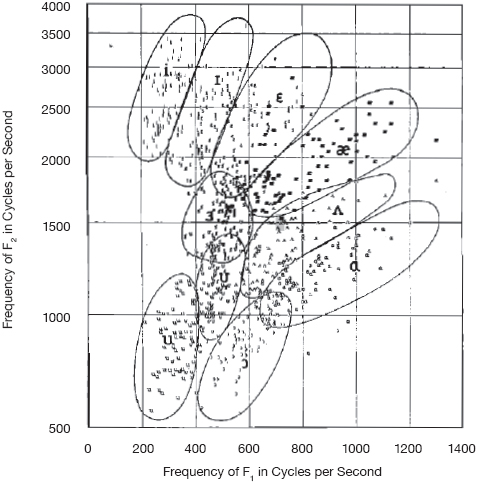
\includegraphics[height=3in]{pg23.jpg}}
\end{frame}

\begin{frame}
  \frametitle{First Formant Resonator}

  When you look at a speech waveform, $x[n]$, most of what you see is
  the first resonance, called the ``first formant.''  Its resonant
  frequency is roughly $400\le F_1\le 800$ usually, so at $F_s=16000$Hz
  sampling frequency, we get
  \[
  \omega_1 = \frac{2\pi F_1}{F_S} \in \left[\frac{\pi}{20},\frac{\pi}{10}\right]
  \]
  Its bandwidth might be about $B_1\approx 400$Hz, so
  \[
  \sigma_1 = \frac{1}{2}\left(\frac{2\pi B_1}{F_s}\right) \approx \frac{\pi}{40}
  \]
\end{frame}

\begin{frame}
  \frametitle{First Formant Frequency and  Bandwidth in the Waveform}

  \centerline{\includegraphics[width=4.5in]{exp/speechwaves.png}}
\end{frame}


\begin{frame}
  \frametitle{First Formant Frequency and  Bandwidth in the Spectrum}

  \centerline{\includegraphics[width=4.5in]{exp/speechspecs.png}}
\end{frame}

%%%%%%%%%%%%%%%%%%%%%%%%%%%%%%%%%%%%%%%%%%%%
\section[Summary]{Summary}
\setcounter{subsection}{1}

\begin{frame}
  \frametitle{Impulse Response of a Second-Order All-Pole Filter}

  A general all-pole filter has the system function
  \[
  H(z) = \frac{1}{(1-p_1z^{-1})(1-p_1^*z^{-1})}= \frac{1}{1-(p_1+p_1^*)z^{-1}+p_1p_1^*z^{-2}}
  \]
  Its impulse response is 
  \[
  h[n] = C_1p_1^n u[n] + C_1^* (p_1^*)^n u[n]
  \]
\end{frame}

\begin{frame}
  \frametitle{Impulse Response of a Second-Order All-Pole Filter}

  We can take advantage of complex numbers to write these as
  \[
  H(z) = \frac{1}{1-2e^{-\sigma_1}\cos(\omega_1)z^{-1}+ e^{-2\sigma_1}z^{-2}}
  \]
  and
  \[
  h[n] = \frac{1}{\sin(\omega_1)} e^{-\sigma_1n}\sin(\omega_1(n+1)) u[n]
  \]
\end{frame}

\begin{frame}
  \frametitle{Magnitude Response of a Second-Order All-Pole Filter}

  In the frequency response, there are three frequencies that really matter:
  \begin{enumerate}
  \item Right at the pole, at $\omega=\omega_1$, we have
    \begin{displaymath}
      |H(\omega_1)| \propto \frac{1}{\sigma_1}
    \end{displaymath}
  \item At $\pm$ half a bandwidth, $\omega=\omega_1\pm\sigma_1$, we have
    \begin{displaymath}
      |H(\omega_1\pm\sigma_1)| =\frac{1}{\sqrt{2}}|H(\omega_1)|
    \end{displaymath}
  \end{enumerate}
\end{frame}  

\end{document}
